\pagebreak
\chapter{Methods}
\label{sec:methods}

\section{Pipeline Overview}

The procedure followed in the current work is displayed in figure \autoref{fig:pipeline}.

\begin{figure}[htbp]
    \centering
    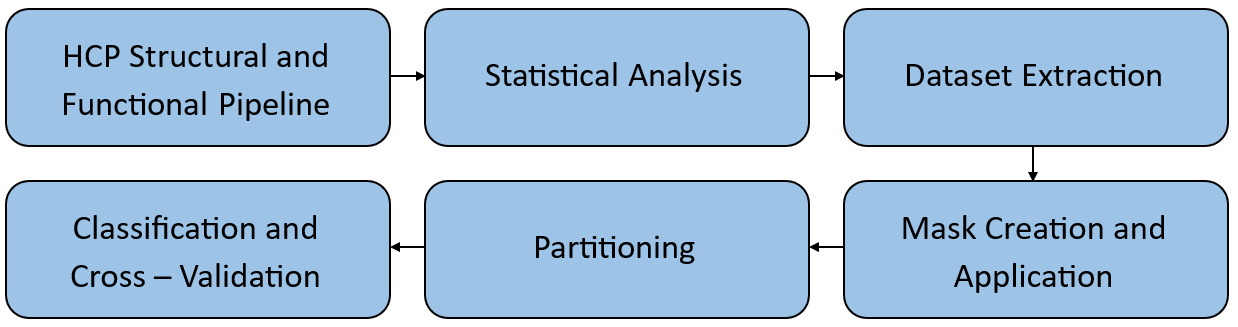
\includegraphics[width = 0.75\textwidth]{assets/images/pipeline.png}
    \caption[Pipeline Overview]{Pipeline Overview.}
    \label{fig:pipeline}
\end{figure}

\begin{wrapfigure}{r}{0.4\textwidth}
    \centering
    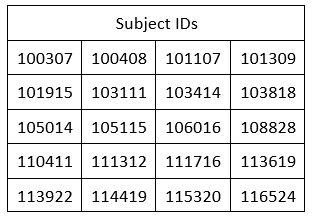
\includegraphics[width = 0.4\textwidth]{assets/images/IDs.png}
    \caption[]{List of IDs for subjects initially chosen for all analyses.}
    \label{fig:ids}
\end{wrapfigure}

% Manually add to the List of Tables and lower list of figures counter.
\addtocounter{table}{1}
\addcontentsline{lot}{table}{\protect\numberline{\thetable}Analysis Subject IDs}
\addtocounter{figure}{-1}

The starting point of the data was preprocessed \gls{WM} task \gls{fMRI} \gls{NIfTI} files, which had undergone initial pre-processing steps included in the structural and then functional \gls{HCP} pipelines \cite{Glasser2013} and were downloaded from the ConnectomeDB platform \cite{ConnectomeDB}. Twenty subjects, selected arbitrarily to balance a reasonable effect size with low computing power needs, were included as shown in figure \autoref{fig:ids}. For all analyses, \gls{NIfTI} files from both \gls{LR} and \gls{RL} scans were included for all subjects. This \gls{LR} and \gls{RL} distinction was made to facilitate geometric distortion correction while simultaneously providing additional data points.

\section{Pipeline Segments}

\subsection{Preprocessing}

All data processing was executed in FMRIB Software Library, abbreviated FSL (FSL v. 6.0.7.12, \cite{Jenkinson2012}). A single preprocessing setting was altered from those in the \gls{HCP} pipelines: the spatial smoothing parameter. The dimensions of the rectangular smoothed voxel neighborhoods were changed from \SI{5}{\milli\meter} to \SI{4}{\milli\meter}. This adjustment improves the singal-to-noise ratio and is a widely used standard for relatively small \gls{ROI}s, such as the \gls{FFA} and \gls{PPA}, which are examined in this study.

\subsection{Statistical Analysis}
\label{subs:stat}

Voxel-wise time-series were input into \gls{FEAT}. Based on the eight \gls{EV}s established by the \gls{HCP} pipeline (.fsf files) --- two \gls{EV}s for each stimulus category, one for 2-Back and one for 0-Back trials --- new \gls{COPE}s were designed. Two different analyses were conducted, both utilizing double-Gamma \gls{HRF} convolution fitting: 

\begin{figure}[htbp]
    \centering
    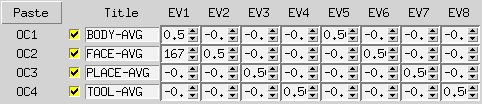
\includegraphics[width = 0.75\textwidth]{assets/images/COPEs_2C.png}
    \caption[]{List of \gls{COPE}s designed for all \gls{2C} analyses.}
    \label{fig:copes_2C}
\end{figure}

% Manually add to the List of Tables and lower list of figures counter.
\addtocounter{table}{1}
\addcontentsline{lot}{table}{\protect\numberline{\thetable}2C Analyses COPEs}
\addtocounter{figure}{-1}

\begin{enumerate}[label=\Roman*.]

\item In the first analysis, 4 \gls{COPE}s (see fig. \autoref{fig:copes_2C}) were parametrized to estimate the \gls{HRF} corresponding to the average \gls{BOLD} signal of each stimulus category, regardless of the N-Back paradigm used. The category-specific signal was averaged by including both 2-Back and 0-Back trials with equal weighting ($ 50 - 50 $), and the signal from all other trials was subtracted using a factor of $ -0.167$ $(1/6)$.

\item In the second case, the same approach was taken, but the signals from 2-Back and 0-Back trials for each stimulus category were considered independent, resulting in 8 \gls{COPE}s (see fig. \autoref{fig:copes_4C}). This decision was based on the fact that these blocks were always separated by tens of seconds. Thus, each \gls{EV}'s average signal was calculated while subtracting all other sources with a factor of $ -0.143$ $(1/7)$.

\end{enumerate}

\begin{figure}[htbp]
    \centering
    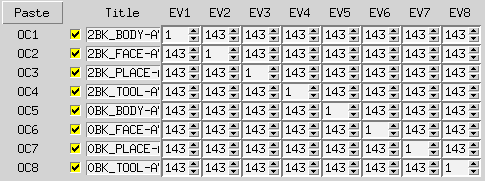
\includegraphics[width = 0.75\textwidth]{assets/images/COPEs_4C.png}
    \caption[]{List of \gls{COPE}s designed for all \gls{4C} analyses.}
    \label{fig:copes_4C}
\end{figure}

% Manually add to the List of Tables and lower list of figures counter.
\addtocounter{table}{1}
\addcontentsline{lot}{table}{\protect\numberline{\thetable}4C Analyses COPEs}
\addtocounter{figure}{-1}

A Unix shell script was created to automate \acrshort{FEAT} analyses across all runs of all available subjects. The script requires only the original .fsf file, which contains the analysis design, as input. In the first case, each analysis produced $4$ \gls{COPE}s, resulting in $4$ patterns per run (\gls{LR} and \gls{RL}) and $8$ patterns per subject, generating a total of $160$ patterns. In the second case, each analysis produced $8$ \gls{COPE}s, resulting in $8$ patterns per run (\gls{LR} and \gls{RL}) and $16$ patterns per subject, generating a total of $320$ patterns.

It is important to note that the \acrshort{FEAT} analysis is a single core process and the time required to complete is not bound on the number of \gls{COPE}s included, but rather on the complexity of the \gls{COPE} design and the quantity of voxels analysed. As a result, with the current hardware limitations and no parallel programming automation designed for this body of work, each analysis took an average of approximately 22 \si{\minute} in the first occasion and 16 \si{\minute} in the second, even though the number of \gls{COPE}s was doubled in the latter.

\subsection{Dataset Extraction - Construciton}

All subsequent data analysis was conducted using custom code written in MATLAB (R2023b). A script was developed to extract patterns from each run for each subject, scalable to accommodate any name and number of subjects. All patterns were conjoined into a single dataset, with sample attributes assigned to them, including target, target label and chunk. The target refers to the stimulus category, numbered as follows: 1 for Body, 2 for Face, 3 for Place, and 4 for Tool, with the labels being the human-readable target names. Chunks are distinguished by a unique number, denoting pattern independence. This independence is crucial because it allows the classifier to train and test on disjoint sets of chunks, thereby avoiding circular analysis (double-dipping).

The analysis that merges signal from 2-Back and 0-Back trials resulted in $2$ chunks per subject and shall be referred to as analysis \gls{2C}. The analysis that separates the signals from different N-Back paradigms produced $4$ chunks per subject and will therefore be called \gls{4C}.

\subsection{Mask Creation - Application}

Once the data was fully processed, two masks were created to distinguish data pertaining to the \gls{FFA} and the \gls{PPA}. These masks, which are logical matrices applied to the dataset to exclude any data outside the selected \gls{ROI}, were "circular", though pixelated, with a radius of $12$ voxels, containing a total of $1,416$ voxels. Mask centers were determined using Neurosynth's Locations Tool (see \cite{neurosynth}) and identified as [40, -52, -20] for the \gls{FFA} and [26, -33, -19] for the \gls{PPA}, in MNI152 coordinates. The radius was specifically chosen to maximize \gls{ROI} volume (ensuring the intended brain region is within the \gls{ROI} for all subjects) while preventing overlap between brain regions that process different category-specific information, as shown in figure (\autoref{fig:radius}).

\begin{figure}[htbp]
    \centering
    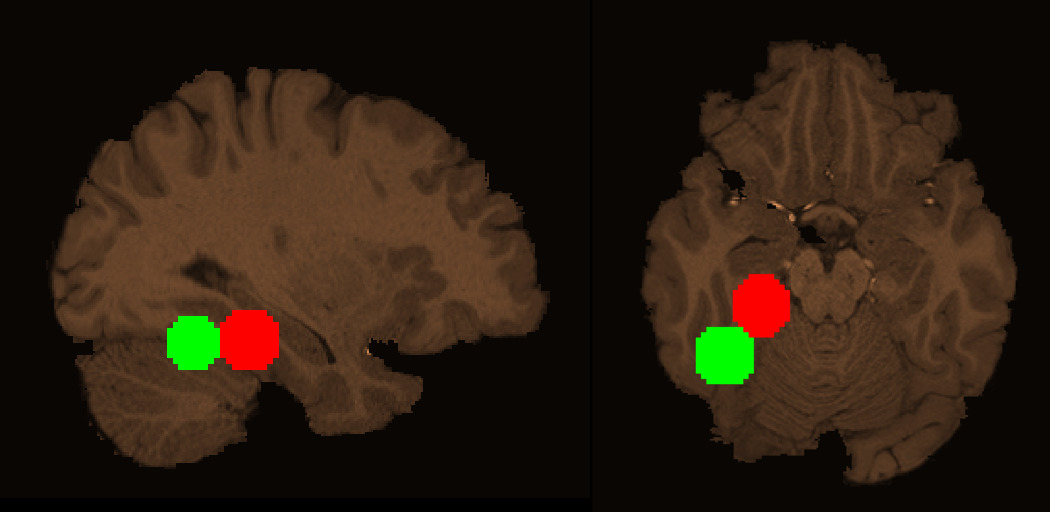
\includegraphics[width = 0.75\textwidth]{assets/images/masks_sag_trans.jpg}
    \caption[Illustration of FFA and PPA masks]{Illustration of \gls{FFA} and \gls{PPA} \gls{ROI}s after mask application, at the saggital and transverse planes. Notably, there is no overlap between the two areas, even when they are at their maximum extent.}
    \label{fig:radius}
\end{figure}

It should be noted that this is the first point at which the sheer volume of data can be reduced without loss of potentially crucial information. The initial dataset contained patterns for all $902.629$ voxels, depicting signal for the entire brain. After the \gls{FFA} and \gls{PPA} masks were applied, the non-zero signal voxels included in the masked datasets were $925$ and $888$ respectively, allowing for a much faster, more efficient and more intricate manipulation of the data.

\subsection{Partitioning of Masked Dataset}

For classification, the data must be split into independent training and test sets. A script was developed to partition the masked dataset with a variable train/test split ratio. To facilitate cross-validation, the script can produce a specified number of folds, each containing unique combinations of patterns within training and test datasets. The classifier can be run on any number of these partitions, resulting in a mean accuracy that reliably reflects the classifier's predictive ability, independent of any single partitioning scheme. Partitioning was conducted with the CoSMo \gls{MVPA} independent\_sample\_partitioner command \cite{cosmo1}, following the appropriate manipulation of the dataset.

\subsection{Classifier Training and Testing \textit{(MVPA)}}

Classification is a supervised machine learning method in which the model predicts the correct label for a given input based on an algorithm that recognizes patterns associated with each label. In this study, the classifier functions as an 'eager learner,' creating a model and making future predictions based on this model, rather than continuously comparing test data to training data. A descriptive illustration of the process can be seen in \autoref{fig:class}.

\begin{figure}[htbp]
    \centering
    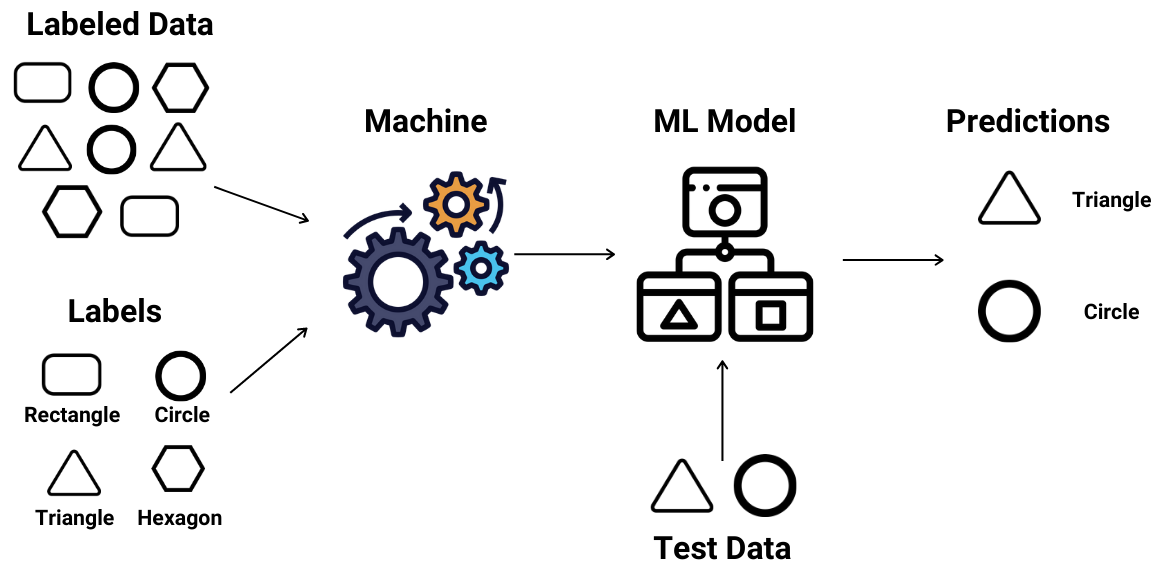
\includegraphics[width = 0.75\textwidth]{assets/images/class.png}
    \caption[Illustration of Supervised Learning Classification]{Supervised Learning Classificaiton Illustration. Adapted from \cite{ML}.}
    \label{fig:class}
\end{figure}

In this case, classification was conducted using the CoSMo \gls{MVPA} cosmo\_classify\_libsvm command \cite{cosmo2} which utilizes a \gls{SVM}  algorithm \cite{Cortes1995}.

\section{Data Analysis}

The classifier's accuracy was treated as a function of three variables, with all other parameters staying constant. The three variables were: 1) number of chunks of data per subject; 2) fold count; and 3) subject count.

\subsection{Category-Secific Baseline Brain Activation \textit{(UPA)}}

\glsreset{UPA}
The first step in facilitating further analysis is the \gls{UPA} of the baseline brain activation signal for each stimulus category in both regions. For each region, the statistical b-value assigned to each cope after the \acrshort{FEAT} analysis was used as an indicator of the baseline signal magnitude. The mean of the square of all values associated with each stimulus category was calculated to account for both positive and negative values. Consequently, the means for all \gls{2C} analyses were derived from 40 patterns, while for \gls{4C}, they were derived from 80 patterns, corresponding to the number of target-pattern pairs in each dataset. The results were presented in bar plots.

Additionally, an extra analysis was conducted for the \gls{FFA}, using cope values derived from a \acrshort{FEAT} analysis of a smaller, more central \gls{FFA} region with a radius of 6 voxels around the center, compared to the 12-voxel radius used previously. This approach aimed to clarify the relationships among the various signals, as they are expected to be more robust in this more focused area.

\subsection{Classifier Performance - Chunks per Subject}
\label{subs:ch_per_subj}

The \gls{WM} task paradigm used in the \gls{HCP} limits the maximum number of chunks per subject to 4, as trials within the same stimulation block (without intermittent fixation blocks) cannot be considered independent, and subjects participated in a total of 4 active trial blocks. However, the minimum number of chunks per subject can be as low as 1, effectively treating all trials as subject-dependent. The choice of chunk count depends on the researcher's approach and objectives.

\begin{enumerate}[label=\Roman*.]

\item In analysis \gls{4C} all blocks were considered independent as long as they involved a different N-Back paradigm and were separated by at least one fixation block. A total of 80 chunks were assigned to the 320 patterns, with each chunk containing 4 patterns, one for each target.

\item In analysis \gls{2C} the N-Back paradigm restriction was lifted. Signal from the same target's 2-Back and 0-Back blocks was placed in the same chunk, resulting in 40 chunks for all 320 patterns, with each chunk containing 8 patterns. Essentially, these chunks represent different runs, with two for each subject, totaling 40 chunks.

\end{enumerate}

\subsection{Detecting Outlier Subjects}
\label{subs:outliers}

The first step in data manipulation following \gls{FEAT} analyses was to identify any individual subjects whose data stood out as irregular. Considering our analysis focuses on the Fusiform Gyrus in the right hemisphere only, subjects who predominantly show activation in the left hemisphere could potentially dilute the classifier's data pool. The same issue can arise if a subject's data acquisition process contained artifacts. Determining outlier subjects is crucial before proceeding with further data analysis steps in order for the results to be reflective of the truth.

The 16 patterns corresponding to each subject in analysis \gls{4C} were individually run through the classifier, cross-validated with the maximum fold count of 4. In this process, 3 chunks (each containing 4 patterns) were used as training data, while the remaining chunk was utilized for testing. The mean accuracy of the classifier across all folds was calculated, and if it fell below 10\%, the subject was excluded from the remainder of the analysis, since such low accuracy is attributed to the nature of the data and not the classifier's properties. Consequently, two subjects were excluded from both the \gls{FFA} and the \gls{PPA} analyses, as further explained in \autoref{subs:res_outliers_ffa}.

These subject exclusions were applied to analysis \gls{2C} as well. Although the approach differs between N-Back trials for the same category-specific stimulus, the classifier's input remains fundamentally the same, so the characteristics that define a subject as an outlier are expected to remain consistent. Moreover, replicating the same analysis for \gls{2C} is impractical since each subject corresponds to only 8 patterns divided into 2 chunks. At best, this would allow for a 50/50 train/test split, where each dataset contains 4 patterns from different chunks. This split is far from ideal and does not accurately reflect the classifier's performance under the 80/20 ratio, which is utilized for all analyses to follow.

\subsection{Classifier Performance - Fold Count}

Cross-validation is essential for verifying the classifier's results, but it can also lengthen and complicate the process by introducing another variable: fold count. It's crucial to investigate this variable to determine the optimal number of folds for practical, repetitive analyses, as well as to identify the smallest number of folds at which the classifier's performance stabilizes. This allows us to estimate the maximum time required, even for high-precision analyses, ensuring efficiency without compromising accuracy.

Initially, \gls{4C} data was run through the classifier for all 18 subjects at high fold counts, starting at 250 and increasing up to 3000 in steps of 250 folds. The objective was to identify the cutoff point where performance stabilizes and further increasing the fold count no longer yields benefits. The accuracy metric at this stabilization point will be considered the objective accuracy of the classifier, serving as the benchmark to aim for at lower fold counts as well. Once the benchmark was established, the data was rerun through the classifier at fold counts ranging from 10 to 100. This approach not only highlights the classifier's performance at low, and therefore practical, fold counts but also helps identify the fold count at which the distribution of partitioning schemes closely resembles the one that produces the benchmark accuracy value. This allows for a more efficient yet accurate analysis by balancing practicality with precision. The same process was then repeated for \gls{2C} data. The optimal fold count was determined to be 68 folds for analysis \gls{4C} and 69 folds for analysis \gls{2C}. 

\subsection{Classifier Performance - Subject Count}

Another crucial variable to consider is the subject count. While accuracy is generally expected to improve as the number of subjects increases, provided they have been screened for outliers as shown in \autoref{subs:outliers}, it's important to determine the exact relationship between accuracy and subject count --- whether it is linear or more complex. Additionally, identifying if and when performance reaches an asymptote, and at what subject count or chunk count this practically occurs, is essential for optimizing the analysis without unnecessarily increasing the sample size.

A script was developed to automate the classification process for both \gls{4C} and \gls{2C} analyses across varying subject counts. For \gls{4C}, data from 1 to 18 subjects were sequentially fed into the classifier. When more than 2 subjects were involved, the optimal fold count of 68 was maintained. For 1 and 2 subjects, the fold count was set to the maximum possible, which was 4 and 28, respectively.

For \gls{2C}, the analysis for a single subject was skipped due to the limitations imposed by having only 2 chunks. The fold count was then set to 4, 15, 28, 45, and 66 for 2, 3, 4, 5, and 6 subjects, respectively, reflecting the maximum feasible number of folds for those subject counts. For all other subject counts, the fold count was standardized at 69.